\documentclass[main.tex]{subfiles}
\begin{document}
\chapter{Quantum chromodynamics in practice}
\label{chapter:qcd}
    In the previous chapter we introduced the basic concepts
    of QCD and setup the framework of calculating
    cross-sections. Cross-sections are the most relevant
    quantities to compute as they can be measured
    experimentally, and are a property of the particles
    being collided, rather than depending on the
    specifics of the experimental procedure.
    This provides a bridge to compare
    theoretical predictions and experimental measurements.
    The relevant quantity calculated in perturbation theory
    is the partonic cross-section which
    is the matrix element integrated over the relevant
    final-state phase-space, normalised by a flux factor.
    The matrix elements are
    calculated order-by-order in the strong coupling
    $\alpha_{s}$ (c.f. \ref{eqn:matrix_element}),
    where each order corresponds to a set of Feynman diagrams
    that have the appropriate number of vertices,
    as each QCD vertex brings along a factor of $\alpha_{s}$.

    In this chapter we will discuss the problems that
    arise when evaluating these Feynman diagrams and outline
    some solutions that have been widely adopted to circumvent
    these issues in order to provide real-world applicable predictions.
    This chapter forms the theoretical foundations upon which
    this thesis is built on.

    We will consider the divergent nature of matrix
    elements and introduce the most widely used techniques
    to tame these singularities.

\section{Divergent structures}\label{sec:divergences}
    The computation of matrix elements essentially reduces down
    to evaluating Feynman diagrams which are analytical expressions
    built up from the Feynman rules of a theory (c.f. QCD Feynman rules
    \ref{fig:qcd_feynman_rules}). In evaluating certain
    topologies of Feynman diagrams, integral expressions
    containing unconstrained momenta will give rise to
    singularities. The divergences
    associated with high energy modes are ultraviolet
    (UV) divergences and on the opposite end of the energy
    spectrum, low energy modes give rise to 
    infrared (IR) divergences.

    The de-facto methods to alleviate these
    divergences are through regularisation
    for UV divergences, and through subtraction
    schemes for IR divergences. Both of these
    methods will be discussed in this section.

\subsection{Ultraviolet divergences}\label{sec:UV}
    During intermediate steps of calculations,
    such as the compututation of loop diagrams seen in
    Figure~\ref{fig:bubble_diagram},
    we have to evaluate integrals of the form
    \begin{equation}\label{eqn:loop_integral}
        I_{\mathrm{UV}} = \int_{0}^{\Lambda} \dfrac{\mathrm{d}^{4}\ell}{(2\pi)^{4}}\dfrac{1}{\ell^{2}(\ell+p)^{2}} \sim \log{\Lambda} \, ,
    \end{equation}
    where a cutoff scale $\Lambda$ has been introduced to
    capture the divergence as the loop momenta
    $\ell \rightarrow \infty$. It is clear that the
    integral diverges in this high energy limit,
    hence the name ultraviolet divergence.
    This UV divergence cannot influence the
    experimentally observable quantities at experiments,
    which are finite, because the final observable
    should not depend on the intermediate steps taken
    to get there.
    Infinities associated with UV divergences
    are removed via the process of renormalisation
    which introduces counterterms in the Lagrangian
    to exactly cancel these divergences.

    \begin{figure}
        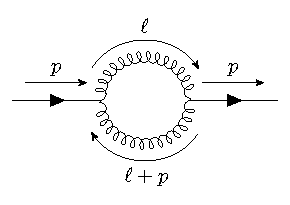
\includegraphics[scale=1.2]{qcd/bubble_diagram.pdf}
        \caption{Massless bubble diagram which is an example of where unconstrained
        loop momenta can lead to UV divergences.}
        \label{fig:bubble_diagram}
    \end{figure}

    Before we introduce these counterterms, we
    first consider the procedure of regularisation
    which makes these infinities explicitly manifest.
    The most widely adopted method of regularisation
    is dimensional regularisation (DR) \cite{tHooft:1972tcz} which
    is based on the observation that the integral
    (\ref{eqn:loop_integral}), which is carried
    out in $d=4$ space-time dimensions, would be finite
    if $d < 4$.

    In DR we define $d = 4 - 2\epsilon$ such that
    after Feynman parametrisation (\ref{eqn:loop_integral})
    becomes
    \begin{equation}\label{eqn:dim_reg}
        I_{\mathrm{UV}} = \int \dfrac{\mathrm{d}^{d}\ell}{(2\pi)^{d}}\dfrac{1}{\ell^{2}(\ell+p)^{2}} = \dfrac{\mathrm{i}}{(4\pi)^{2}}\left(\dfrac{-p^{2}}{4\pi}\right)^{-\epsilon}\dfrac{\Gamma(1-\epsilon)^{2}}{\Gamma(2-2\epsilon)} \, \Gamma(\epsilon) \, ,
    \end{equation}
    where the divergence for $d = 4$, or equivalently
    $\epsilon \rightarrow 0$, is now captured in the
    Gamma function, $\Gamma(\epsilon)$. This becomes clear once
    we expand $\Gamma(\epsilon)$ around small $\epsilon$
    \begin{equation}\label{eqn:gamma_laurent}
        \Gamma(\epsilon) = \dfrac{1}{\epsilon} - \gamma_{E} + \dfrac{1}{2}\left(\gamma_{E}^{2} + \dfrac{\pi^{2}}{6}\right)\epsilon + \mathcal{O}(\epsilon^{2}) \, ,
    \end{equation}
    where $\gamma_{E} \approx 0.577$ is the Euler-Mascheroni
    constant, meaning the divergence is now regularised as a pole in
    $\epsilon$.

\subsection{Renormalisation}\label{sec:renormalisation}
    With the UV divergence regularised by dimensional
    regularisation, it is now possible to construct the
    counterterms order-by-order in $\alpha_{s}$ to
    explicitly cancel the divergences.

    A subtlety with adjusting the dimension of the theory
    from $d=4$ to arbitrary dimensions is that the mass dimension
    of the Lagrangian has to change accordingly to retain a
    dimensionless action in natural units. We can account for this by
    introducing an arbitrary energy scale $\mu_{R}$, the renormalisation
    scale, into the gauge coupling
    constant to modify the mass dimension of the Lagrangian.
    For QCD this is done via the modification
    \begin{equation}\label{eqn:dimensionful_coupling}
        g_{s} \rightarrow g_{s}\mu_{R}^{\epsilon} \, .
    \end{equation}
    where it is understood that the original gauge coupling is
    dimensionless. The order of $\mu_{R}$ is determined by examining
    the dimensions of the gauge and fermion fields
    in the Lagrangian (\ref{eqn:L_QCD}).
    We see that this introduces a scale dependence
    on the coupling constant $\alpha_{s}$, a point we will return
    to in Section~\ref{sec:alpha_running}.
    % In a calculation,
    % intermediate steps will have a dependence on $\mu$,
    % however, once the $\epsilon \rightarrow 0$ limit
    % is taken the scale dependence drops out.

    The inclusion of counterterms into the theory can be
    thought of as renormalisations of the bare fields
    and couplings in the QCD Lagrangian (\ref{eqn:L_QCD}) to restore predictive
    power to the theory. The renormalised fields and couplings
    can be given as (see for instance Ref.~\cite{mangano1999introduction})
    \begin{align}\label{eqn:renormlised_fields}
        \psi_{\mathrm{bare}} &= \sqrt{Z_{2}} \psi_{R} \, , \nonumber \\
        A_{\mathrm{bare}}^{\mu} &= \sqrt{Z_{3}} A_{R}^{\mu} \, ,\\
        g_{s,\mathrm{bare}} &= Z_{g} \mu_{R}^{\epsilon} g_{s,R} \, , \nonumber
    \end{align}
    where it conventional to define $Z_{1} = Z_{g}Z_{2}\sqrt{Z_{3}}$
    such that we can set $Z_{n} = 1 + \delta_{n}$ for $n \in \{1, 2, 3\}$.
    In this way we can write the Lagrangian as
    \begin{equation}
        \mathcal{L}_{R} = \mathcal{L}_{\mathrm{bare}} + \mathcal{L}_{\mathrm{c.t.}} \, ,
    \end{equation}
    where the counterterms appearing in $\mathcal{L}_{\mathrm{c.t.}}$
    are determined by calculating $\delta_{n}$. There is freedom
    in the choice of $\delta_{n}$ which gives rise to
    different regularisation schemes. The minimal subtraction
    (MS) scheme subtracts only the epsilon pole appearing
    in loop integrals. However, the most
    commonly used regularisation scheme is the modified minimal
    subtraction ($\overline{\mathrm{MS}}$) scheme which subtracts the
    epsilon pole plus a universal constant appearing in all
    loop integrals.

    In an all orders calculation of an observable,
    there would be no dependence on the renormalisation
    scale as it is a remnant of the regularisation prescription
    However, because in perturbative QCD observables
    are calculated order-by-order, there will be a residual
    dependence on the renormalisation scale stemming from
    the missing higher order terms. The conventional way
    that the community estimates the uncertainty associated
    with this residual dependence is by carrying out
    a scale variation (see Section~\ref{sec:scale_variations}).

\subsection{Running of the coupling constant}\label{sec:alpha_running}
    The renormalisation scale introduced during regularisation
    is a mathematical artifact and should not impact any measurable
    quantities. Therefore, the bare coupling should not depend on
    the renormalisation scale,
    \begin{equation}\label{eqn:d_g_bare_d_mu}
        \dfrac{\mathrm{d}g_{s,\mathrm{bare}}}{\mathrm{d}\mu_{R}} = 0 \, ,
    \end{equation}
    or said another way, the renormalisation process
    is independent of the actual value of the renormalisation scale.
    The consequence of this is that the renormalised coupling, $\alpha_{s}(\mu_{R})$, has to
    depend on the renormalisation scale instead.

    The renormalisation scale dependence of $\alpha_{s}$
    is governed by the Callan-Symanzik \cite{Callan:1970yg,Symanzik:1970rt}
    $\beta$-function
    \begin{equation}\label{eqn:beta_fn}
        \mu_{R}^{2} \dfrac{\partial \alpha_{s}(\mu_{R}^{2})}{\partial \mu_{R}^{2}} = \beta(\alpha_{s}) \, ,
    \end{equation}
    where the $\beta$-function can be written as a perturbative
    expansion in $\alpha_{s}$
    \begin{equation}\label{eqn:beta_series}
        -\beta(\alpha_{s}) = \alpha_{s}\sum_{n=0}^{\infty}\left(\dfrac{\alpha_{s}}{4\pi}\right)^{n+1} \beta_{n}\, 
    \end{equation}
    where the coefficients $\beta_{n}$ have been computed
    up to $\beta_{4}$ \cite{Baikov:2016tgj,Luthe:2017ttg}.
    The solution to (\ref{eqn:beta_fn}) to first order
    is
    \begin{equation}\label{eqn:1l_alpha}
        \alpha_{s}(\mu_{R}^{2}) = \dfrac{1}{\frac{\beta_{0}}{4\pi}\log\left(\frac{\mu_{R}^{2}}{\Lambda_{\mathrm{QCD}}^{2}}\right)} \, ,
    \end{equation}
    where $\Lambda_{\mathrm{QCD}}$ is the QCD scale,
    the scale at which $\alpha_{s}$ becomes
    large enough that perturbation theory breaks down,
    and $\beta_{0} = (11C_{A} - 4T_{R}n_{f})/3$.
    In QCD, $C_{A}=3$ and $T_{R}=\frac{1}{2}$, meaning for
    $n_{f} < \frac{33}{2}$ the sign of $\beta_{0}$ is positive.
    In nature we have observed six flavours of quarks, so
    $\beta_{0} > 0$. In fact all $\beta$-coefficients
    computed to date are positive, meaning that $\alpha_{s}$
    decreases with increasing energy due to the minus sign
    in (\ref{eqn:beta_series}). This property is known as
    asymptotic freedom \cite{Gross:1973id,Politzer:1973fx},
    and is justification for treating QCD perturbatively
    when the energy scale is high, such as at collider experiments.
    The running of the coupling constant has been
    observed experimentally as illustrated in Figure~\ref{fig:alpha_s_running}.

    \begin{figure}
        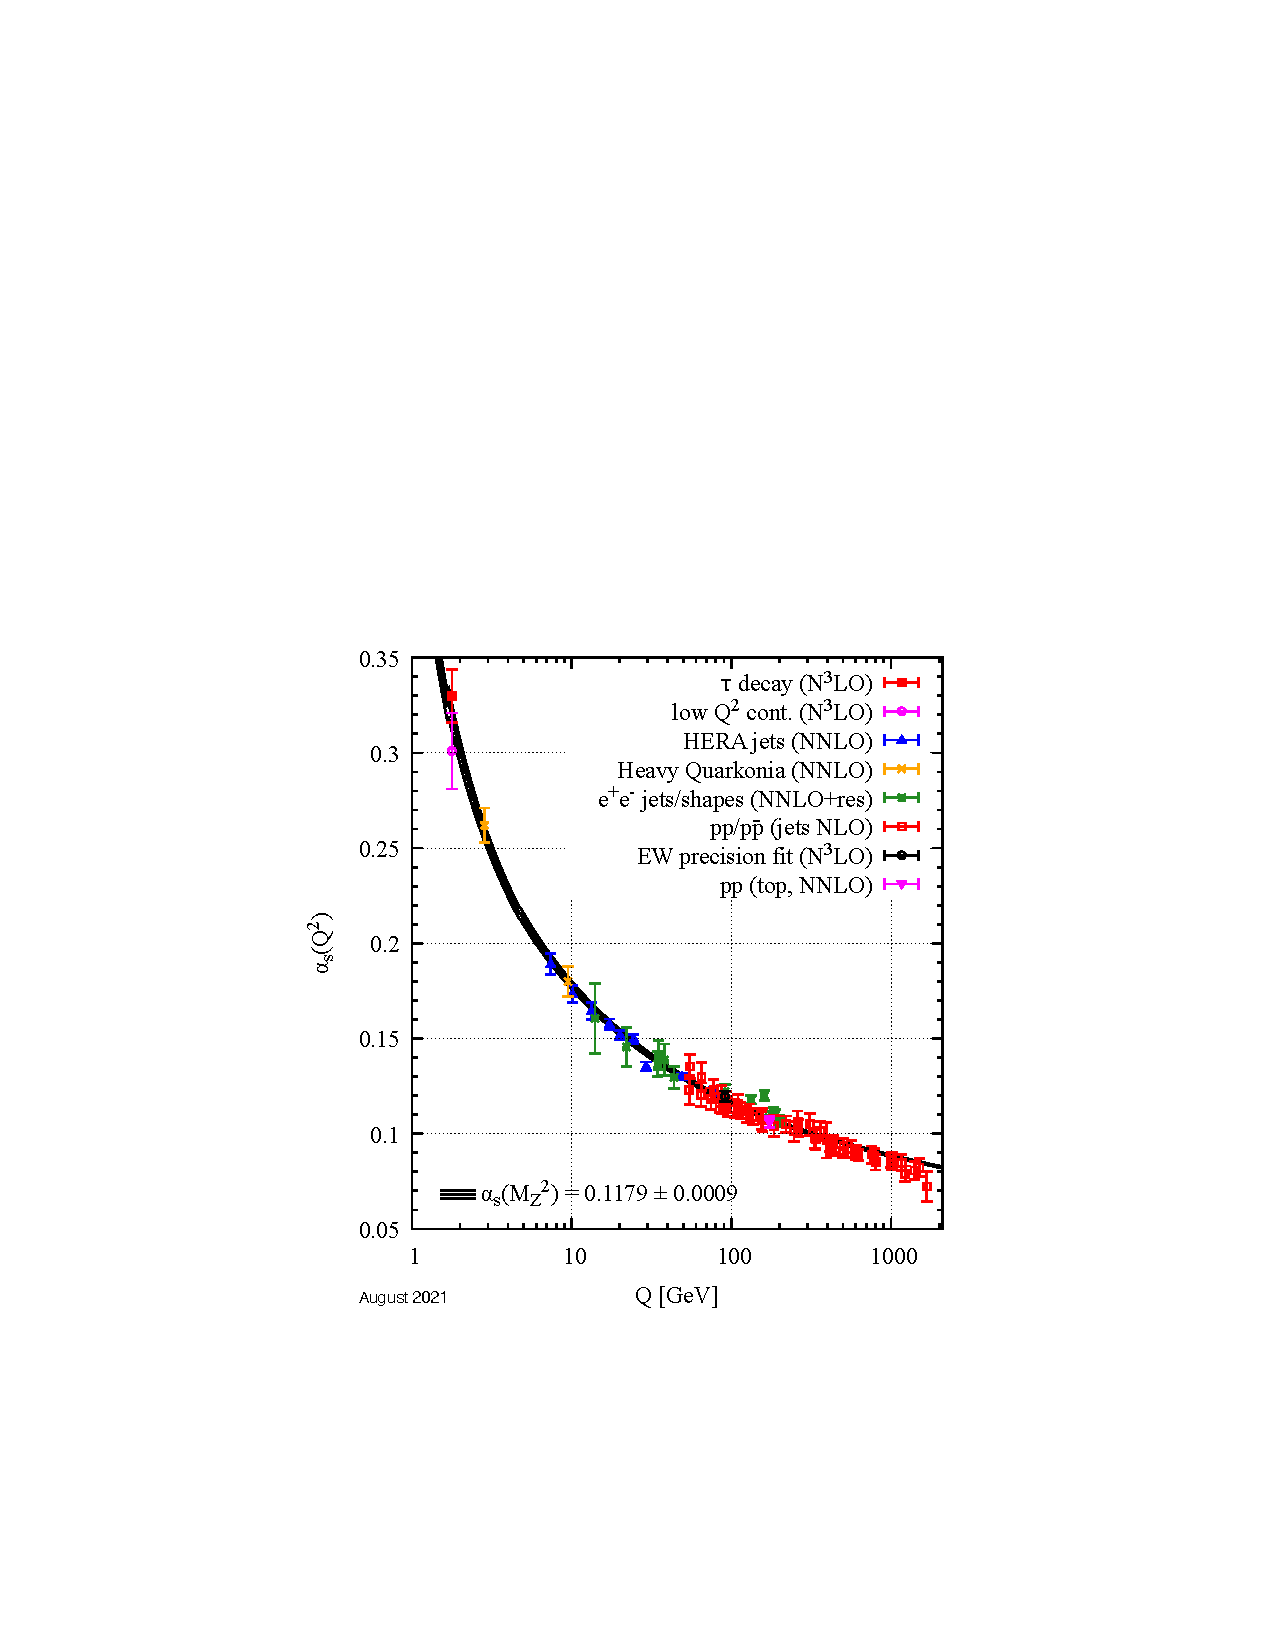
\includegraphics{qcd/alpha_s_running.pdf}
        \caption{The running of the strong coupling constant $\alpha_{s}$,
        as determined by experiments, with QCD theory prediction in black.
        Figure reference \cite{Workman:2022ynf}.}
        \label{fig:alpha_s_running}
    \end{figure}

    Another consequence of the running coupling
    is colour confinement, in which quarks and
    gluons cannot exist as free particles. Due
    to the increasing strength of coupling at low
    energies, quarks and gluons are forced to
    form composite, colourless particles. This means
    that at low energies, perturbative QCD
    is not an accurate description of nature,
    and the behaviour of hadrons cannot be predicted
    from perturbation theory. Instead phenomenological
    models have to be used to describe these processes.
    
\subsection{Infrared divergences}\label{sec:IR_divergences}
    In Section~\ref{sec:UV} we saw how divergences
    stemming from high energy behaviour would occur
    in loop diagrams. On the other end of the energy
    spectrum we also have divergences from low energy
    modes. Since these divergences emerge from low energy
    behaviour they are called infrared (IR) divergences. There
    are two cases in which these divergences arise:
    \begin{itemize}
        \item virtual divergences in loop integrals,
        \item real emission divergences when an emission
    of an extra particle has vanishing energy (soft),
    or becomes parallel to an external leg (collinear).
    \end{itemize}

    Virtual IR divergences can be understood by looking
    at an integral of the form
    \begin{equation}\label{eqn:virtual_IR_integral}
        I_{\mathrm{V}} = \int \dfrac{\mathrm{d}^{4}\ell}{(2\pi)^{4}} \dfrac{1}{\ell^{2}(\ell+p_{1})^{2}(\ell-p_{2})^{2}} \, ,
    \end{equation}
    which is encountered when calculating the one-loop
    virtual correction to the gluon-quark-antiquark vertex
    as shown in Figure~\ref{fig:vertex_correction}.
    It is clear that the denominator vanishes when $\ell \rightarrow 0$
    or when either $(\ell + p_{1})^{2}$ or $(\ell - p_{2})^{2} \rightarrow 0$.
    These situations correspond to the gluon in the loop propagator
    going soft, or collinear to the external quark or antiquark.
    These divergences are regulated in DR to give
    \begin{equation}\label{eqn:virtual_IR_DR}
        I_{\mathrm{V}} = \dfrac{\mathrm{i}}{(4\pi)^{2}Q^{2}}\left(\dfrac{-Q^{2}}{4\pi}\right)^{-\epsilon}\dfrac{\Gamma(1+\epsilon)\Gamma(1-\epsilon)^{2}}{\Gamma(1-2\epsilon)}\left[\dfrac{1}{\epsilon^{2}}\right] \, ,
    \end{equation}
    where $Q = (p_{1} + p_{2})$. There is a double $\epsilon$ pole manifest,
    corresponding to the soft and collinear divergence.

    \begin{figure}
        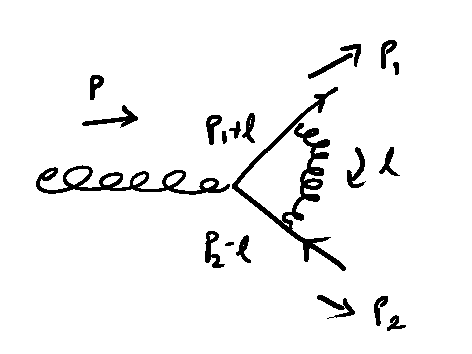
\includegraphics[scale=1.2]{qcd/vertex_correction.pdf}
        \caption{One-loop vertex correction for the gluon-quark-antiquark vertex which diverges
        for $\ell \rightarrow 0$.}
        \label{fig:vertex_correction}
    \end{figure}

    Real IR divergences are manifest when integrating
    matrix elements over the phase-space of external state momenta.
    Matrix elements can be written as functions of Mandelstam variables
    \begin{equation}\label{eqn:mandelstam}
        s_{ij} = (p_{i} + p_{j})^{2} \xrightarrow[\mathrm{limit}]{\mathrm{massless}} 2 E_{i}E_{j}(1-\cos \theta_{ij}) \, ,
    \end{equation}
    where $p_{i}$ and $p_{j}$ are the 4-momenta of partons $i$ and $j$
    in the hard scattering.
    When either of the partons beecome soft, $E_{i,j}\rightarrow 0$,
    or when they go collinear to each other, $\theta_{ij} \rightarrow 0$,
    the matrix element will diverge if $s_{ij}$ appears
    in the demoninator. These scenarios correspond to an external
    particle becoming unresolved.

    In Section~\ref{sec:renormalisation}, we removed UV divergences
    through the use of counterterms to renormalise the theory, making
    predictions from the theory physical.
    IR divergences, on the other hand, arise even after the theory
    has been renormalised. The resolution to IR divergences is given by the
    Block-Nordsieck \cite{Bloch:1937pw,Yennie:1961ad} and Kinoshita-Lee-Nauenberg
    (KLN) theorems \cite{Kinoshita:1962ur,Lee:1964is} which states
    that at each order of perturbation theory, the virtual and real
    contributions exactly cancel out, leaving only finite corrections.
    This cancellation occurs because the infrared pole structure is
    identical in the real and virtual corrections, but with an opposite sign.

    At a detector of a collider experiment, there is a finite
    energy resolution of the calorimeter. This means that
    it is not physically possible to observe arbitrarily soft
    partons. It is also not possible to distinguish two partons
    at arbitrarily small angles from one parton with the combined
    momenta. These limitations along with the KLN theorem
    means that any physical observable that we wish to predict
    with fixed-order perturbation theory must be insensitive to the
    emissions of soft or collinear partons. Any observable obeying
    this criteria is an infrared and collinear (IRC) safe observable.
    This leads to the concept of jets \cite{Salam:2010nqg} which are collimated
    particles combined according to some jet algorithm.    

    In DR, the singularities from soft and collinear divergences
    are manifest as $\epsilon$ poles which makes the cancellation
    simple between the real and virtual parts. However, in practice, 
    the phase-space integrals of the matrix elements are rarely carried
    out analytically due to the high dimensionality of the integral,
    rendering them intractable.
    Instead they are done numerically through the use
    of Monte Carlo methods (see Chapter~\ref{chap:MC}),
    which requires the integral to be in
    integer dimensions. Therefore, numerical techniques
    have been developed to deal with these IR divergences as well. The
    most common technique, subtraction, will be discussed in
    more detail in Section~\ref{sec:subtraction}.
    
\section{Factorisation of matrix elements}\label{sec:me_factorisation}
    In the previous section we examined the IR divergences
    that can arise in matrix elements, either explicitly
    through loop diagrams, or implicitly when carrying
    out the phase-space integral over the external state
    momenta. In this section we will discuss how these IR
    singularities are universal and how the divergences
    associated with real emissions can be factorised out
    of the matrix element. This property is exploited
    extensively in Chapters~\ref{chapter:fame1}, \ref{chapter:fame2},
    and \ref{chapter:fame3}
    where the research of this thesis is presented.

    The regions of phase-space in which real emission
    matrix elements diverge are when the emission is
    soft and/or collinear. It can be shown that in these
    regions of phase-space, the matrix element factorises
    into a process-independent singular factor, multiplied
    by a matrix element with the unresolved parton
    being absorbed by an emitting leg -- we call this the reduced matrix
    element. This factorisation, however, is not exact
    in QCD where there are spin and colour correlations.

    Schematically, the $(n+1)$-body matrix element
    factorises as
    \begin{equation}\label{eqn:me_factorisation}
        |\mathcal{M}_{n+1}|^{2} \rightarrow \bm{S}_{ijk} \otimes |\mathcal{M}_{n}|^{2} \, ,
    \end{equation}
    where $\bm{S}_{ijk}$ is a universal singular factor capturing
    the IR divergent behaviour and $|\mathcal{M}_{n}|^{2}$
    is the reduced matrix element. The $\otimes$
    represents the colour and spin correlations existing
    between the singular function and the reduced matrix element.
    This singular factor
    is not unique and can be represented by different
    approximations as long as they reproduce the
    correct IR behaviour. In this thesis we discuss
    two approximations: Catani-Seymour dipoles \cite{Catani:1996vz}
    in Section~\ref{sec:CS_dipoles} and antenna functions \cite{Gehrmann-DeRidder:2005btv}
    in Section~\ref{sec:antenna_functions}. The indices
    of $\bm{S}_{ijk}$ already hints at the fact that the singular
    functions only depends on three partons, and not all
    of the external states.

    We will inspect the soft and collinear limits separately
    to see how the matrix element factorises in these respective
    limits.
    The following section will follow the conventions
    of Ref.~\cite{Catani:1996vz}, namely that the colour and
    helicity summed $n$-body matrix element written as
    \begin{equation}\label{eqn:CS_matrix_element}
        |\mathcal{M}_{n}|^{2} = {}_{n}\langle 1, \ldots, n | 1, \ldots, n \rangle_{n}
    \end{equation}
    where $| 1, \ldots, n \rangle_{n}$ is a vector
    in colour + helicity space (see Appendix~\ref{appendix:catani_seymour}
    for a more thorough explanation on notation).

\subsection{Soft limits}\label{sec:me_soft}
    Consider a tree-level matrix element $|\mathcal{M}_{n+1}|^{2}$
    with a final-state gluon $j$. Note that reduced matrix
    elements associated with taking a quark soft have to vanish
    due to violation of quark number, therefore only gluons
    are considered.
    The limit of the soft gluon with momentum
    $p_{j}$ can be parametrised by
    \begin{equation}\label{eqn:soft_parametrisation}
        p_{j}^{\mu} = \lambda q^{\mu} \, , \quad \lambda \rightarrow 0 \, ,
    \end{equation}
    where $q^{\mu}$ is an arbitrary four-vector and $\lambda$
    is a scale parameter. In this limit the matrix element
    can be written as
    \begin{equation}\label{eqn:soft_factorisation}
        \begin{split}
        |\mathcal{M}_{n+1}|^{2} \rightarrow &-\dfrac{1}{\lambda^{2}}8\pi \mu^{2\epsilon}\alpha_{s} \sum_{i}\dfrac{1}{p_{i}q} \sum_{k \neq i} \dfrac{p_{k}p_{i}}{(p_{i} + p_{k})q} \\
        &{}_{n}\langle 1, \ldots, j-1, j+1, \ldots, n+1 | \bm{T}_{k} \cdot \bm{T}_{i} | 1, \ldots, j-1, j+1, \ldots, n+1 \rangle_{n} \, ,
        \end{split}
    \end{equation}
    where terms less singular than $1 / \lambda^{2}$ have been
    neglected. The reduced matrix element represented by the
    colour + helicity vector inner product is obtained by removing
    the soft gluon from the $(n+1)$-body matrix element.
    The indices $i$, $j$, and $k$ label partons involved
    in the factorsation process: $i$ is the emitter parton,
    $j$ is the emitted parton, and $k$ is a parton accounting
    for the colour correlations. The scale $\mu$ can be identified as the
    renormalisation scale, and $\bm{T_{i}}$ is the colour-charge
    operator. It acts on the colour vectors in the reduced matrix element
    to give factors of $C_{A}$ and $C_{F}$, hence this factorisation is not exact.

    The matrix elements in (\ref{eqn:soft_factorisation}) are
    unambiguously defined only when momentum conservation is
    fulfilled. This is only true in the strict $\lambda = 0$
    limit. Away from the limit, care has to be taken to conserve
    momentum conservation and keep the relevant partons on-shell.
    This can be done through the use of momentum mappings
    \cite{Catani:1996vz,Kosower:1997zr}.

\subsection{Collinear limits}\label{sec:me_collinear}
    For the collinear limit, consider partons $i$ and
    $j$ in the matrix element $|\mathcal{M}_{n+1}|^{2}$.
    Their momenta can be decomposed as
    \begin{align}\label{eqn:F_collinear_momenta}
        \begin{split}
        p_{i}^{\mu} &= z p^{\mu} + k_{\perp}^{\mu} - \dfrac{k_{\perp}^{2}}{z} \dfrac{n^{\mu}}{2 p \cdot n} \, \\
        p_{j}^{\mu} &= (1-z) p^{\mu} - k_{\perp}^{\mu} - \dfrac{k_{\perp}^{2}}{1-z}\dfrac{n^{\mu}}{2 p \cdot n} \, , 
        \end{split}
    \end{align}
    where $p^{\mu}$ denotes the collinear direction
    of the two partons, $k_{\perp}^{\mu}$ specifies
    the transverse direction perpendicular to the
    collinear direciton ($p \cdot k_{\perp} = 0$), and $n^{\mu}$ is an auxiliary
    vector satisfying the conditions $n^{2} = 0$ and $k_{\perp} \cdot n = 0$.
    $z$ is the fraction of momenta carried away from
    the collinear momentum by parton $i$.
    
    The collinear limit can be then be defined as
    \begin{equation}\label{eqn:F_collinear limit}
        2 p_{i} p_{j} = s_{ij} = - \dfrac{k_{\perp}^{2}}{z(1-z)} \, , \quad k_{\perp} \rightarrow 0 \, .
    \end{equation}
    In this limit the matrix element can be written as
    \begin{equation}\label{eqn:F_collinear_factorisation}
        |\mathcal{M}_{n+1}|^{2} \rightarrow \dfrac{1}{p_{i}p_{j}}4\pi \mu^{2\epsilon}\alpha_{s} \; {}_{n} \langle 1, \ldots, ij, \ldots, n+1 | \hat{P}_{ij}(z, k_{\perp}) | 1, \ldots, ij, \ldots, n+1 \rangle_{n} \, ,
    \end{equation}
    where terms less singular than $k_{\perp}^{2}$ have been neglected.
    This reduced matrix element is obtained by replacing the partons
    $i$ and $j$ with a single parton $ij$ which carries the
    momentum $p^{\mu}$ and suitable quantum numbers depending
    on the partons $i$ and $j$. For example, if $i =$ quark and $j=$ gluon,
    then $ij =$ quark, or if $i=$ quark and $j =$ antiquark, then $ij =$ gluon.
    $\hat{P}_{ij}$ are the $d$-dimensional Altarelli-Parisi splitting
    functions that depend on the momentum fraction $z$ for the splitting
    $ij \rightarrow i + j$ and the transverse momentum $k_{\perp}$.
    Each splitting function is a matrix acting on the spin indices of $ij$.
    Due to these spin correlations the reduced matrix
    element does not factorise from the splitting functions exactly.

    $\hat{P}_{ij}$ become the more recognisable Altarelli-Parisi
    splitting functions (\ref{eqn:AP_kernels}) once spin-averaged
    and the $\epsilon \rightarrow 0$ limit is taken.

    In general, it is possible for a final-state
    parton $i$ to become collinear with an initial-state parton $a$.
    This is described by the splitting process $a \rightarrow ai + i$.
    In this case their momenta can be decomposed as
    \begin{align}\label{eqn:I_collinear_momenta}
        \begin{split}
        p_{i}^{\mu} &= (1-x)p_{a}^{\mu} + k_{\perp}^{\mu} - \dfrac{k_{\perp}^{2}}{1-x}\dfrac{n^{\mu}}{2p_{a} \cdot n} \, , \\
        p_{a}^{\mu} &= x p_{a}^{\mu} \, ,
        \end{split}
    \end{align}
    with the collinear limit defined as
    \begin{equation}\label{eqn:I_collinear_limit}
        2p_{i}p_{a} = s_{ia} = -\dfrac{k_{\perp}^{2}}{1-x} \, , \quad k_{\perp} \rightarrow 0 \, .
    \end{equation}

    The analogous expression of (\ref{eqn:F_collinear_factorisation})
    for initial-state splitting is
    \begin{equation}\label{eqn:I_collinear_factorisation}
        |\mathcal{M}_{n+1}|^{2} \rightarrow \dfrac{1}{x} \dfrac{1}{p_{i}p_{a}} 4\pi \mu^{2\epsilon} \alpha_{s} \; {}_{n} \langle 1,\ldots,n+1;ai, \ldots | \hat{P}_{ai}(x, k_{\perp}) | 1,\ldots,n+1;ai,\ldots \rangle_{n} \, ,
    \end{equation}
    where the replacement of partons $a$ and $i$ have been made
    explicit by the presence of the parton $ai$ in the colour + helicity vector.
    The specific type of parton $ai$ depends upon the types of $a$ and $i$.

    Similar to (\ref{eqn:soft_factorisation}) where the factorisation was
    only true in the strict soft limit, (\ref{eqn:F_collinear_factorisation})
    and (\ref{eqn:I_collinear_factorisation}) are only
    true in the strict collinear limit. Away from these
    limits care has to be taken to conserve momenta
    via the use of momenta mappings.

\subsection{Factorisation of colour-ordered amplitudes}\label{sec:CO_factorisation}
    The factorisation formulae expressed in (\ref{eqn:soft_factorisation}),
    (\ref{eqn:F_collinear_factorisation}), and (\ref{eqn:I_collinear_factorisation})
    were not exact because of colour and spin correlations.
    It can be shown that the factorisation of matrix
    elements in the soft and collinear limits becomes
    exact once the colour structure of the gauge group
    is separated from the kinematics. 

    In general any QCD amplitude can be
    colour decomposed, that is the colour structure is
    separated from the kinematics. Consider the process $e^{+}e^{-} \rightarrow q\bar{q} + n \; g$
    \footnote{For the scope of this thesis it is sufficient
    to consider colour decomposition of electron-positron
    annihilation into a single quark pair plus gluons,
    and not the more general case of multiple quark
    flavours in the final-state.},
    the amplitude can be written as a product of hadronic and
    leptonic currents \cite{Campbell:1998nn}
    \begin{equation}\label{eqn:epem_amplitude}
        \mathcal{M}(q_{1}, \bar{q}_{2}; 1, \ldots, n) = \hat{\mathcal{S}}_{\mu}^{n+2}(q_{1}; 1,\ldots,n; \bar{q}_{2})V^{\mu} \, ,
    \end{equation}
    where $V^{\mu}$ is the leptonic current and the hadronic
    current is
    \begin{equation}\label{eqn:hadronic_current}
        \hat{\mathcal{S}}_{\mu}^{n+2}(q_{1};1,\ldots,n;\bar{q}_{2}) = \mathrm{i}eg_{s}^{n} \sum_{P(1,\ldots,n)}(T^{a_{1}} \ldots T^{a_{n}})_{c_{1}c_{2}}S_{\mu}(q_{1};1,\ldots,n;\bar{q}_{2}) \, .
    \end{equation}
    In this expression we have the electromagnetic gauge coupling
    $e$ and the strong gauge coupling $g_{s}$ appearing. The colour
    structure has been factorised into a product of fundamental group
    generators where the indices $a_{i} \in \{1,\ldots, N_{c}^{2}-1\}$
    and $c_{i} \in \{1,\ldots,N_{c}\}$. This leaves the colour-ordered
    partial amplitude $S_{\mu}(q_{1};1,\ldots,n;\bar{q}_{2})$ depending
    only on kinematical variables. In this partial amplitude, the gluons
    are emitted in an ordered fashion from the quarks, meaning the quarks
    have a fixed position in the partial amplitude.
    The sum over $P(1,\ldots,n)$ represents the sum over all permutations
    of gluon emissions which accounts for all Feynman diagrams and colour structures.

    Upon squaring the amplitude (\ref{eqn:epem_amplitude}), we get
    \begin{equation}\label{eqn:epem_me2}
        \left|\hat{\mathcal{S}}_{\mu}^{n+2}V^{\mu}\right|^{2} = e^{2}\left(\dfrac{g_{s}^{2}N_{c}}{2}\right)^{n}\left(\dfrac{N_{c}^{2}-1}{N_{c}}\right) \sum_{P(1,\ldots,n)} \left(\left|S_{\mu}(q_{1};1,\ldots,n;\bar{q}_{2})V^{\mu}\right|^{2} + \mathcal{O}\left(\dfrac{1}{N_{c}^{2}}\right)\right) \, ,
    \end{equation}
    where the subleading colour terms proportional to $1/N_{c}^{2}$ have been omitted.
    The first term in the sum is the leading colour term
    and is the dominant term in the colour expansion.

    With the amplitude written in terms of the colour-ordered
    partial amplitudes, it is now possible to factorise (\ref{eqn:epem_me2})
    exactly in the soft and collinear limits. Consider the limit where a final-state
    gluon $j$ is soft, we have
    \begin{equation}\label{eqn:CO_soft_factorisation}
        \left|S_{\mu}(q_{1};1,\ldots,i,j,k,\ldots,n;\bar{q}_{2})V^{\mu}\right|^{2} \rightarrow S_{ijk} \left|S_{\mu}(q_{1};1,\ldots,i,k,\ldots,n;\bar{q}_{2})V^{\mu}\right|^{2} \, ,
    \end{equation}
    where the factor
    \begin{equation}\label{eqn:eikonal_factor}
        S_{ijk} = 4\dfrac{s_{ik}}{s_{ij}s_{jk}} \, ,
    \end{equation}
    is the well-known eikonal factor. We see that the colour-ordered
    amplitude on the RHS of (\ref{eqn:CO_soft_factorisation}) has gluon $j$
    removed but the ordering of all hard partons remain unchanged.

    In the collinear limit where partons $i$ and $j$ become collinear
    to form parton $k$, the matrix element factorises as
    \begin{equation}\label{eqn:CO_collinear_factorisation}
        \left|S_{\mu}(q_{1};1,\ldots,i,j,\ldots,n;\bar{q}_{2})V^{\mu}\right|^{2} \rightarrow \dfrac{2}{s_{ij}}P_{ij}(z) \left|S_{\mu}(q_{1};1,\ldots,k,\ldots,n;\bar{q}_{2})V^{\mu}\right|^{2} \, ,
    \end{equation}
    where $P_{ij}(z)$ are the spin-averaged Altarelli-Parisi splitting
    functions (\ref{eqn:AP_kernels}) with the colour factors removed.
    In this expression it is understood that the indices $i$, $j$, and $k$
    have to be self-consistent for the different partonic splittings.
    For partons which are not colour connected (are not neighbouring
    partons in the colour-ordered amplitude), there will be no singular
    behaviour as $s_{ij} \rightarrow 0$.

    In (\ref{eqn:CO_soft_factorisation}) and (\ref{eqn:CO_collinear_factorisation})
    the colour-ordered amplitude factorises exactly into a
    colour-ordered amplitude with one parton removed, multiplied
    by a universal singular factor. This singular factor depends on the unresolved
    parton and the two neighbouring hard particles. Interpreting this as
    the two hard particles forming an antenna which radiates the unresolved
    parton gives rise to the antenna functions which will be discussed
    further in Section~\ref{sec:antenna_functions}.

\subsection{One-loop matrix element factorisation}\label{sec:OL_factorisation}
    The discussion of matrix element factorisation so
    far has been focused on tree-level matrix elements.
    It has been shown that one-loop colour-ordered amplitudes
    also factorise in the soft and collinear limits \cite{Bern:1994zx,Bern:1998sc,Kosower:1999xi}.
    At the one-loop level, there are new universal singular
    functions and the factorisation formulae are modified.

    In the soft limit, a one-loop colour-ordered amplitude
    factorises as
    \begin{equation}\label{eqn:1L_soft_factorisation}
        M_{n+1}^{(1)}(\ldots, i, j, k, \ldots) \rightarrow S_{ijk}^{(0)} \, M_{n}^{1}(\ldots, i, k, \ldots) + S_{ijk}^{(1)}(\epsilon) \, M_{n}^{0}(\ldots, i, k, \ldots) \, ,
    \end{equation}
    where $S_{ijk}^{(0)}$ is the eikonal factor (\ref{eqn:eikonal_factor}),
    and $S_{ijk}^{(1)}(\epsilon)$ is the one-loop soft radiation function \cite{Bern:1999ry}.

    A similar factorisation formula for the collinear limit is
    \begin{equation}\label{eqn:1L_collinear_factorisation}
        M_{n+1}^{(1)}(\ldots, i, j, \ldots) \rightarrow \dfrac{1}{s_{ij}} \left[ P_{ij}^{(0)}(z) \, M_{n}^{(1)}(\ldots, k, \ldots) + P_{ij}^{(1)}(z, \epsilon) \, M_{n}^{(0)}(\ldots, k, \ldots) \right] \, ,
    \end{equation}
    where $P_{ij}^{(0)}(z)$ are the tree-level splitting functions
    (\ref{eqn:AP_kernels}) and $P_{ij}^{(1)}(z, \epsilon)$
    are the one-loop splitting functions \cite{Bern:1999ry}.

    In both these formulae the structure is of the form:
    tree-level splitting function multipled by a one-loop
    amplitude, plus a one-loop splitting function multiplied
    by a tree-level amplitude.

    In Section~\ref{sec:antenna_functions} we will give
    a brief overview of antenna functions where these one-loop
    factorisation formulae were used to obtain universal singular functions
    at the one-loop level for squared matrix elements. These
    antenna functions are then applied in the context of NLO
    k-factor emulation in Chapter~\ref{chapter:fame2}.

\section{Subtraction}\label{sec:subtraction}
    In Section~\ref{sec:IR_divergences} we discussed the
    structure of IR divergences and how the KLN theorem
    necessitated the cancellation of IR divergences 
    arising from the virtual corrections and real-emission
    matrix elements once integrated over soft and collinear
    regions of phase-space, at each order in perturbation
    theory.

    Over the past few decades there has been a vast
    amount of research into devising methods to systematically
    isolate these singularities such that it is possible
    to make finite predictions of physical quantities numerically.
    To tackle this problem, three
    main methods have been proposed: phase-space slicing \cite{Fabricius:1981sx,Kramer:1986mc,Giele:1991vf},
    sector decomposition \cite{Binoth:2000ps,Binoth:2003ak}, and subtraction \cite{Ellis:1980nc}.
    
    By now the method of choice at NLO QCD is subtraction,
    and is the method we will focus on in this section. The main
    idea behind subtraction methods is to define local counterterms
    that exactly replicate the IR divergent behaviour of matrix
    elements. While there is not one single subtraction scheme
    that is universally used, the general form of a subtraction term
    must fulfill the requirements of replicating the matrix element
    behaviour in all IR singular limits, and be analytically integrable
    over the regions of phase-space corresponding to these IR limits.

    To illustrate the idea behind the subtraction method,
    first consider the calculation of a LO partonic cross-section
    \begin{equation}\label{eqn:LO_cs}
        \sigma^{\mathrm{LO}} = \int \mathrm{d}\Phi_{n} \; \mathcal{B}_{n} \, ,
    \end{equation}
    where $\mathcal{B}_{n}$ is the Born (tree-level) matrix
    element and $\Phi_{n}$ is the $n$-body phase-space.
    At the next order in perturbation theory, we have the NLO
    cross-section which recieves contributions from the real and virtual
    corrections
    \begin{equation}\label{eqn:NLO_cs}
        \sigma^{\mathrm{NLO}} = \int \mathrm{d}\Phi_{n} \; \left[\mathcal{B}_{n} + \mathcal{V}_{n}\right] + \int \mathrm{d}\Phi_{n+1} \; \mathcal{R}_{n+1} \, ,
    \end{equation}
    where $\mathcal{V}_{n}$ is the virtual matrix element (renormalised
    to remove UV divergences as described in Section~\ref{sec:UV})
    which lives in the same $n$-body phase-space as the Born
    matrix element. The real-emission matrix element, $\mathcal{R}_{n+1}$,
    lives in the $(n+1)$-body phase-space, $\Phi_{n+1}$, due to the emission
    of an additional external particle. The integrals over $\Phi_{n}$ and
    $\Phi_{n+1}$ are separately divergent but their sum is finite. To
    carry out a numerical calculation, it is therefore necessary
    to regulate these divergences to make them explicit.
    Using dimensional regularisation these
    divergences are mapped to poles in $\epsilon$.

    The motivation behind the subtraction method is that the
    divergences in (\ref{eqn:NLO_cs}) can be cancelled upon the insertion
    of a counterterm evaluated in $\Phi_{n+1}$, $\mathcal{C}_{n+1}$,
    and an integrated counterterm evaluated in $\Phi_{n}$, $\mathcal{I}_{n}$,
    such that the condition
    \begin{equation}\label{eqn:subtraction_term_condition}
        \int \mathrm{d}\Phi_{n} \; \mathcal{I}_{n} - \int \mathrm{d}\Phi_{n+1} \; \mathcal{C}_{n+1} = 0 \, ,
    \end{equation}
    holds. Here phase-space factorisation is utilised:
    $\Phi_{n+1} \rightarrow \Phi_{n}\Phi_{1}$ when using
    an appropriate $3 \rightarrow 2$ momentum mapping \cite{Catani:1996vz,Kosower:2002su} such that
    \begin{equation}\label{eqn:integrated_counterterm}
        \mathcal{I}_{n} = \int \Phi_{1} \; \mathcal{C}_{n+1} \, ,
    \end{equation}
    where $\Phi_{1}$ is the one-parton phase-space leading
    to $\epsilon$ poles once $\mathcal{C}_{n+1}$ is integrated over.
    The counterterm $\mathcal{C}_{n+1}$ should be a proper
    pointwise approximation of $\mathcal{R}_{n+1}$ to cancel all IR
    divergences such that $\mathcal{R}_{n+1} - \mathcal{C}_{n+1}$ is finite.
    Additionally, since the pole structure in $\mathcal{V}_{n}$ is identical
    to $\mathcal{R}_{n+1}$ but with an opposite sign, $\mathcal{V}_{n} + \mathcal{I}_{n}$ will be finite
    by construction.
    Inserting the subtraction terms into (\ref{eqn:NLO_cs}) we get
    \begin{equation}\label{eqn:NLO_subtraction}
        \sigma^{\mathrm{NLO}} = \int \mathrm{d}\Phi_{n} \left[\mathcal{B}_{n} + \mathcal{V}_{n} + \mathcal{I}_{n}\right] + \int \mathrm{d}\Phi_{n+1} \left[\mathcal{R}_{n+1} - \mathcal{C}_{n+1}\right] \, ,
    \end{equation}
    where each integral can now be carried out numerically
    in integer dimensions by taking the $\epsilon \rightarrow 0$
    limit. This is possible as the integrals are all separately
    finite now.

    The counterterm $\mathcal{C}_{n+1}$ has been kept general
    but specific exmples of automated subtractions schemes include
    Catani-Seymour (CS) \cite{Catani:1996vz,Catani:2002hc},
    Frixione-Kunszt-Signer (FKS) \cite{Frixione:1995ms,Frixione:1997np},
    and antenna subtraction \cite{Campbell:1998nn,Kosower:1997zr,Kosower:2003bh}.

    Beyond NLO QCD, the algorithms available have
    not reached the maturity of the automated methods widely use
    at NLO. However, this is an active area of
    research. See Reference \cite{TorresBobadilla:2020ekr} for a review of methods
    that have been applied to NNLO QCD.

    In the next sections we will describe in detail two sets of functions
    that are used to build subtraction terms: Catani-Seymour dipoles, and
    antenna functions. However, we will not construct the counterterms explicitly.
    In other words, we are interested in the approximations of the matrix elements
    in the soft and collinear limits as these are universal and can
    be applied to any process, and not the subtraction terms themselves.
    These functions will become instrumental
    during our construction of matrix element emulators in Chapters
    \ref{chapter:fame1}, \ref{chapter:fame2}, and \ref{chapter:fame3}.

\section{Catani-Seymour dipoles}\label{sec:CS_dipoles}
    Catani-Seymour dipoles introduced in Ref.~\cite{Catani:1996vz}
    are process-independent functions that reproduce the IR
    singular behaviour of matrix elements. They depend on the
    momenta and quantum numbers of three partons in the real-emission
    phase-space. These three partons are identified by indices
    $i$, $j$, and $k$ where $i$ is the emitting parton, $j$ is
    the unresolved emitted parton, and $k$ is a spectator parton.
    In order to map out all the singular limits in a process, it is
    necessary to construct all permutations of the dipole functions
    since the dipoles only depends on three partons.

    Dipole functions can be separated into four categories
    depending on whether the emitter and spectator are in the
    initial-state or the final-state, as illustrated in Figure~\ref{fig:CS_dipoles}.
    Namely, there are final-final (FF) dipoles, final-initial dipoles (FI),
    initial-final (IF) dipoles and initial-initial (II) dipoles where
    the nomenclature refers to the emitter-spectator dipole.
    For electron-positron annihilations only FF dipoles are required
    since electrons (positrons) do not carry any colour charge
    and so there is no initial-state radiation.
    However, for any hadronic collision the inclusion of the remaining
    dipoles are required to capture all IR-singular behaviour arising
    from the initial-state emissions.

    In the following we will describe in detail the FF dipoles
    and the associated matrix element factorisation formula,
    but only give a brief description of the remaining dipoles as
    the structure of the terms and factorisation formulae
    generalise analogously.

    \begin{figure}
        \centering
        \begin{subfigure}{0.49\linewidth}
            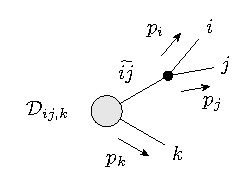
\includegraphics[width=\linewidth]{qcd/Dijk.pdf}
            \caption{FF dipole}
            \vspace{20pt}
        \end{subfigure}
        \begin{subfigure}{0.49\linewidth}
            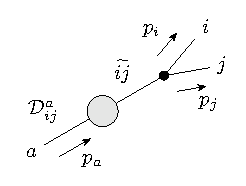
\includegraphics[width=\linewidth]{qcd/Daij.pdf}
            \caption{FI dipole}
            \vspace{20pt}
        \end{subfigure}
        \begin{subfigure}{0.49\linewidth}
            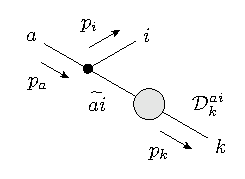
\includegraphics[width=\linewidth]{qcd/Daik.pdf}
            \caption{IF dipole}
        \end{subfigure}
        \begin{subfigure}{0.49\linewidth}
            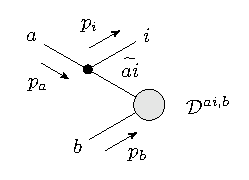
\includegraphics[width=\linewidth]{qcd/Daib.pdf}
            \caption{II dipole}
        \end{subfigure}
        \vspace{30pt}
        \caption{Schematic diagrams of the four classes of Catani-Seymour
            dipoles, $\mathcal{D}$. The dipoles are named according to
            whether the emitter and spectator are in the initial (upper indices) or final-state (lower indices).
            Each dipole consists of a composite particle (denoted by tilde)
            that decays into two partons, and a spectator that recoils
            to conserve momentum. The grey blob represents the hard scattering process,
            with incoming and outgoing lines representing initial- and final-state
            partons, respectively. The black circle represents the splitting
            function within the dipole function which contains the divergent
            behaviour.}
        \label{fig:CS_dipoles}
    \end{figure}

    \subsection{Final-final dipoles}
        The utilisation of dipoles is encapsulated in the
        dipole factorisation formula where matrix elements in the limit
        $p_{i}p_{j} \rightarrow 0$ can be written as
        \begin{equation}\label{eqn:FF_factorisation}
            {}_{n+1} \langle 1, \ldots, n+1 | 1, \ldots, n+1 \rangle_{n+1} = \sum_{i,j}\sum_{k\neq i,j}\mathcal{D}_{ij,k}(p_{1},\ldots,p_{n+1}) + \ldots \, ,
        \end{equation}
        where terms not singular in the limit $p_{i}p_{j} \rightarrow 0$
        are omitted, and the dipole is
        \begin{equation}\label{eqn:D_ijk}
            \begin{split}
                \mathcal{D}_{ij,k}(p_{1},\ldots,p_{n+1}) &= -\dfrac{1}{2p_{i}p_{j}} \\
                {}_{n}\langle 1, &\ldots, \widetilde{ij}, \ldots, \tilde{k}, \ldots, n+1 | \dfrac{\boldsymbol{T}_{k} \cdot \boldsymbol{T}_{ij}}{\boldsymbol{T}_{ij}^{2}} \boldsymbol{V}_{ij,k} | 1, \ldots, \widetilde{ij}, \ldots, \tilde{k}, \ldots, n+1 \rangle_{n} \, ,
            \end{split}
        \end{equation}
        where $\boldsymbol{T}_{i}$ are the colour-charge operators and $\boldsymbol{V}_{ij,k}$
        is a matrix in the helicity space of the emitter embedding the
        IR divergent behaviour.
        The sum in (\ref{eqn:FF_factorisation}) can be understood as summing over all possible
        3 leg permutations to capture all the soft and collinear limits.
        The reduced matrix element on the RHS of (\ref{eqn:D_ijk})
        is obtained by replacing the partons $i$ and $j$ with
        a single parton $\widetilde{ij}$, and replacing parton
        $k$ with a parton $\tilde{k}$. $\tilde{k}$ has all the
        same quantum numbers as $k$, whereas the
        partonic nature of $\widetilde{ij}$ depends on
        the specific splitting process (c.f. Section~\ref{sec:me_collinear}).
        The momenta of these particles are modified in the following way
        \begin{equation}\label{eqn:FF_mapping}
            \tilde{p}_{ij}^{\mu} = p_{i}^{\mu} + p_{j}^{\mu} - \dfrac{y_{ij,k}}{1-y_{ij,k}} p_{k}^{\mu} \, , \quad \tilde{p}_{k}^{\mu} = \dfrac{1}{1-y_{ij,k}}p_{k}^{\mu} \, ,
        \end{equation}
        where $y_{ij,k}$, the recoil parameter, is a dimensionless variable given as
        \begin{equation}\label{eqn:y_ijk}
            y_{ij,k} = \dfrac{p_{i}p_{j}}{p_{i}p_{j} + p_{i}p_{k} + p_{j}p_{k}} \, .
        \end{equation}
        Equations (\ref{eqn:FF_mapping}) and (\ref{eqn:y_ijk})
        are a $3 \rightarrow 2$ momenta mapping that maps
        $p_{i} + p_{j} + p_{k} \rightarrow \tilde{p}_{ij} + \tilde{p}_{k}$.
        The mapping ensures momentum conservation is maintained across all of phase-space and
        all particles are kept on-shell:
        \begin{align}\label{eqn:mapping_conditions}
            \begin{split}
                &p_{i}^{\mu} + p_{j}^{\mu} + p_{k}^{\mu} = \tilde{p}_{ij}^{\mu} + \tilde{p}_{k}^{\mu} \, , \\
                &\tilde{p}_{ij}^{2} = \tilde{p}_{k}^{2} = 0 \, .
            \end{split}
        \end{align}

        The matrices $\boldsymbol{V}_{ij,k}$ are functions of
        $y_{ij,k}$ and the splitting variables $\tilde{z}$
        \begin{equation}\label{eqn:zi}
            \tilde{z}_{i} = \dfrac{p_{i}p_{k}}{p_{i}p_{k} + p_{j}p_{k}} \, , \quad \tilde{z}_{j} = \dfrac{p_{j}p_{k}}{p_{i}p_{k} + p_{j}p_{k}} = 1 - \tilde{z}_{i} \, .
        \end{equation}
        They are analogous to the $z$ from Altarelli-Parisi splitting functions.
        $\boldsymbol{V}_{ij,k}$ acts on the spin indices of the composite particle $\widetilde{ij}$,
        but is independent of the type of the spectator. Making the spin-dependence
        on parton $\widetilde{ij}$ explicit ($s$ and $s'$ for $\widetilde{ij}=\,$fermion, and $\mu$ and $\nu$ for $\widetilde{ij}=\,$gluon)
        we list all the kernels here
        \begin{align}\label{eqn:FF_V_ijk}
            &\langle s | \boldsymbol{V}_{q_{i}g_{j},k} | s' \rangle = 8\pi \mu^{2\epsilon} \alpha_{s} C_{F} \left[\dfrac{2}{1-\tilde{z}_{i}(1-y_{ij,k})} - (1+\tilde{z}_{i}) - \epsilon \tilde{z}_{j} \right] \delta_{ss'} \, , \nonumber \\
            &\langle \mu | \boldsymbol{V}_{q_{i},\bar{q}_{j},k} | \nu \rangle = 8\pi \mu^{2\epsilon} \alpha_{s} T_{R} \left[-g^{\mu\nu} - \dfrac{2}{p_{i}p_{j}}(\tilde{z}_{i}p_{i}^{\mu}-\tilde{z}_{j}p_{j}^{\mu})(\tilde{z}_{i}p_{i}^{\nu}-\tilde{z}_{j}p_{j}^{\nu})\right] \, , \nonumber \\
            \begin{split}
                &\langle \mu | \boldsymbol{V}_{g_{i}g_{j},k} | \nu \rangle = 16\pi \mu^{2\epsilon} \alpha_{s} C_{A} \left[-g^{\mu\nu}\left(\dfrac{1}{1-\tilde{z}_{i}(1-y_{ij,k})} + \dfrac{1}{1-\tilde{z}_{j}(1-y_{ij,k})} - 2\right) \right. \\
                &\hspace{5cm} \left. + \dfrac{(1-\epsilon)}{p_{i}p_{j}}(\tilde{z}_{i}p_{i}^{\mu}-\tilde{z}_{j}p_{j}^{\mu})(\tilde{z}_{i}p_{i}^{\nu}-\tilde{z}_{j}p_{j}^{\nu})\right] \, .
            \end{split}
        \end{align}

        A key feature of these kernels are that they smoothly interpolate
        between the soft and collinear limits, meaning they do not double count
        any limit. Additionally, they only contain divergences in the
        $p_{i}p_{j} \rightarrow 0$ limit and not for any other pair of
        momenta. In the soft and collinear limits, the dipole function
        $\mathcal{D}_{ij,k}$ correctly reproduces the matrix element factorisation
        behaviour seen in (\ref{eqn:soft_factorisation}) and (\ref{eqn:F_collinear_factorisation}),
        repsectively. In particular, $\boldsymbol{V}_{ij,k}$ becomes
        proportional to the eikonal factor and Altarelli-Parisi splitting
        functions in these respective limits.

        In this thesis we will be focussing on the emulation of
        colour- and spin-averaged matrix elements. Therefore the spin-indices
        are not explicitly available. It is possible to average over the spin indices in (\ref{eqn:FF_V_ijk})
        to obtain the spin-averaged splitting functions
        \begin{align}\label{eqn:FF_avg_V_ijk}
            &\langle \boldsymbol{V}_{q_{i}g_{j},k} \rangle = 8\pi \mu^{2\epsilon} \alpha_{s} C_{F} \left[\dfrac{2}{1-\tilde{z}_{i}(1-y_{ij,k})} - (1+\tilde{z}_{i}) - \epsilon \tilde{z}_{j} \right] \, , \nonumber \\
            &\langle \boldsymbol{V}_{q_{i}\bar{q}_{j},k} \rangle = \, 8\pi \mu^{2\epsilon} \alpha_{s} T_{R} \left[1-\dfrac{2\tilde{z}_{i}\tilde{z}_{j}}{1-\epsilon}\right] \, , \nonumber \\
            &\langle \boldsymbol{V}_{g_{i}g_{j},k} \rangle = 16\pi \mu^{2\epsilon} \alpha_{s} C_{A} \left[\dfrac{1}{1-\tilde{z}_{i}(1-y_{ij,k})}+\dfrac{1}{1-\tilde{z}_{j}(1-y_{ij,k})}-2+\tilde{z}_{i}\tilde{z}_{j}\right] \, .
        \end{align}

    \subsection{Final-initial dipoles}
        For the case of final-state emitter and initial-state
        spectator we have the dipole factorisation formula
        \begin{equation}\label{eqn:FI_factorisation}
            \begin{split}
                {}_{n+1}\langle 1, \ldots, n+1; a, \ldots |& 1, \ldots, n+1; a, \ldots \rangle_{n+1} = \\
                &\sum_{i,j}\sum_{k\neq i,j} \mathcal{D}_{ij,k}(p_{1},\ldots,p_{n+1};p_{a},\ldots) \\
                &\sum_{i,j}\sum_{a} \mathcal{D}_{ij}^{a}(p_{1},\ldots,p_{n+1};p_{a},\ldots) + \ldots \, ,
            \end{split}
        \end{equation}
        where the new dipole contribution appears on the second line.
        The initial-state parton is denoted by $a$.
        The dipole term $\mathcal{D}_{ij}^{a}$ is given by
        \begin{equation}\label{eqn:D_aij}
            \begin{split}
                \mathcal{D}_{ij}^{a}(p_{1}, \ldots, p_{n+1}; p_{a}, \ldots) &= -\dfrac{1}{2p_{i}p_{j}} \dfrac{1}{x_{ij,a}} \\
                {}_{n} \langle 1, \ldots, \widetilde{ij}, &\ldots, n+1; \tilde{a}, \ldots | \dfrac{\boldsymbol{T}_{a} \cdot \boldsymbol{T}_{ij}}{\boldsymbol{T}_{ij}^{2}} \boldsymbol{V}_{ij}^{a} | 1, \ldots, \widetilde{ij}, \ldots, n+1; \tilde{a} , \ldots \rangle_{n} \, .
            \end{split}
        \end{equation}
        where $\widetilde{ij}$ is the composite emitter in the
        final-state, and the spectator $\tilde{a}$ is in the initial-state.
        The momentum mapping for $p_{i} + p_{j} + p_{a} \rightarrow \tilde{p}_{ij} + \tilde{p}_{a}$ is given as
        \begin{equation}\label{eqn:FI_mapping}
            \tilde{p}_{ij}^{\mu} = p_{i}^{\mu} + p_{j}^{\mu} - (1-x_{ij,a})p_{a}^{\mu} \, , \quad \tilde{p}_{a}^{\mu} = x_{ij,a} \, p_{a}^{\mu} \, , \\
        \end{equation}
        such that the following momentum conservation and on-shell conditions are met
        \begin{equation}\label{eqn:FI_mapping_conditions}
            \begin{split}
                &p_{i}^{\mu} + p_{j}^{\mu} - p_{a}^{\mu} = \tilde{p}_{ij}^{\mu} - \tilde{p}_{a}^{\mu} \, , \\
                &\tilde{p}_{ij}^{2} = \tilde{p}_{a}^{2} = 0 \, .
            \end{split}
        \end{equation}
        The recoil parameter $x_{ij,a}$ and splitting variables $\tilde{z}$ are given by
        \begin{equation}\label{eqn:x_ija}
        \begin{split}
                &x_{ij,a} = \dfrac{p_{i}p_{a} + p_{j}p_{a} - p_{i}p_{j}}{(p_{i}p_{a} + p_{j}p_{a})} \, , \\
                &\tilde{z}_{i} = \dfrac{p_{i}p_{a}}{p_{i}p_{a} + p_{j}p_{a}} \, , \quad \tilde{z}_{j} = \dfrac{p_{j}p_{a}}{p_{i}p_{a} + p_{j}p_{a}} = 1 - \tilde{z}_{i} \, .
            \end{split}
        \end{equation}
        The spin-averaged splitting functions are given as
        \begin{align}\label{eqn:FI_V_aij}
            &\langle \boldsymbol{V}_{q_{i}g_{j},a} \rangle = 8\pi \mu^{2\epsilon}\alpha_{s} C_{F} \left[\dfrac{2}{1 - \tilde{z}_{i} + (1-x_{ij,a})} - (1+\tilde{z}_{i}) - \epsilon \tilde{z}_{j} \right] \, , \nonumber \\
            &\langle \boldsymbol{V}_{q_{i}\bar{q}_{j},a} \rangle = 8\pi \mu^{2\epsilon}\alpha_{s} T_{R} \, \left[1-\dfrac{2\tilde{z}_{i}\tilde{z}_{j}}{1-\epsilon}\right] \, , \nonumber \\
            &\langle \boldsymbol{V}_{g_{i}g_{j},a} \rangle = 16\pi \mu^{2\epsilon} \alpha_{s} C_{A} \left[\dfrac{1}{\tilde{z}_{j} + (1-x_{ij,a})} + \dfrac{1}{\tilde{z}_{i} + (1-x_{ij,a})} - 2 + \tilde{z}_{i}\tilde{z}_{j}\right] \, .
        \end{align}

    \subsection{Initial-final dipoles}
        For the case of initial-state emitter and final-state spectator,
        the dipole factorisation formula is given as
        \begin{equation}\label{eqn:IF_factorisation}
            {}_{n+1} \langle 1, \ldots, n+1; a | 1, \ldots, n+1; a \rangle_{n+1} = \sum_{a,i}\sum_{k \neq i}\mathcal{D}_{k}^{ai}(p_{1},\ldots,p_{n+1};p_{a}) + \ldots \, ,
        \end{equation}
        where there is only one initial-state parton. The dipole is given by
        \begin{equation}\label{eqn:D_aik}
            \begin{split}
            \mathcal{D}_{k}^{ai}(p_{1}, \ldots, p_{n+1};p_{a}) &= -\dfrac{1}{2p_{a}p_{i}}\dfrac{1}{x_{ik,a}} \\
            {}_{n}\langle 1, \ldots, \tilde{k}, &\ldots, n+1 ; \widetilde{ai} | \dfrac{\boldsymbol{T}_{k} \cdot \boldsymbol{T}_{ai}}{\boldsymbol{T}_{ai}^{2}} \boldsymbol{V}_{k}^{ai} | 1, \ldots, \tilde{k}, \ldots, n+1; \widetilde{ai} \rangle_{n} \, .
            \end{split}
        \end{equation}
        where the emitter is the initial-state parton $\widetilde{ai}$
        and the spectator is the final-state parton $\tilde{k}$.
        The momenta mapping for $p_{a} + p_{i} + p_{k} \rightarrow \tilde{p}_{ai} + \tilde{p}_{k}$ is
        \begin{equation}\label{eqn:IF_mapping}
            \tilde{p}_{ai}^{\mu} = x_{ik,a} \, p_{a}^{\mu} \, , \quad \tilde{p}_{k}^{\mu} = p_{k}^{\mu} + p_{i}^{\mu} - (1-x_{ik,a})p_{a}^{\mu} 
        \end{equation}
        such that
        \begin{equation}\label{eqn:IF_mapping_conditions}
            \begin{split}
            &p_{i}^{\mu} + p_{k}^{\mu} - p_{a}^{\mu} = \tilde{p}_{k}^{\mu} - \tilde{p}_{ai}^{\mu} \, , \\
            &\tilde{p}_{ai}^{2} = \tilde{p}_{k}^{2} = 0 \, .
            \end{split}
        \end{equation}
        Note that the momentum $\tilde{p}_{ai}$ is parallel
        to $p_{a}$, therefore the modified spectator momentum $\tilde{p}_{k}$
        has to recoil the transverse momentum. This leads to $x_{ik,a}$
        acting as a splitting variable.

        With $x_{ik,a}$ taking the role of $\tilde{z}$, there is another
        parameter, $u_{i}$, appearing in the splitting functions.
        These are given as
        \begin{equation}\label{eqn:x_ika}
            x_{ik,a} = \dfrac{p_{k}p_{a}+p_{i}p_{a}-p_{i}p_{k}}{p_{i}p_{a} + p_{k}p_{a}} \, , \quad u_{i} = \dfrac{p_{i}p_{a}}{p_{i}p_{a} + p_{k}p_{a}} \, .
        \end{equation}

        The spin-averaged splitting functions are
        \begin{align}\label{eqn:V_aik}
            &\langle \boldsymbol{V}_{k}^{q_{a}g_{i}} \rangle = \dfrac{n_{s}(q)}{n_{s}(\tilde{q})} \; 8\pi \mu^{2\epsilon} \alpha_{s} C_{F} \left[\dfrac{2}{1-x_{ik,a} + u_{i}} + (1+x_{ik,a}) - \epsilon(1-x_{ik,a})\right] \, , \nonumber \\
            &\langle \boldsymbol{V}_{k}^{g_{a}\bar{q}_{i}} \rangle = \dfrac{n_{s}(g)}{n_{s}(\tilde{q})} \; 8\pi \mu^{2\epsilon} \alpha_{s} T_{R} \left[1 - \dfrac{2x_{ik,a}(1-x_{ik,a})}{1-\epsilon}\right] \, , \nonumber \\
            &\langle \boldsymbol{V}_{k}^{g_{a}g_{i}} \rangle = \dfrac{n_{s}(g)}{n_{s}(\tilde{g})} \; 16\pi \mu^{2\epsilon} \alpha_{s} C_{A} \left[\dfrac{1}{1-x_{ik,a} + u_{i}} + \dfrac{1-x_{ik,a}}{x_{ik,a}} - 1 + x_{ik,a}(1-x_{ik,a}) \right] \, , \nonumber \\
            &\langle \boldsymbol{V}_{k}^{q_{a}q_{i}} \rangle = \dfrac{n_{s}(q)}{n_{s}(\tilde{g})} \; 8\pi \mu^{2\epsilon} \alpha_{s} C_{F} \left[(1-\epsilon)x_{ik,a} + 2\dfrac{1-x_{ik,a}}{x_{ik,a}} \right] \, ,
        \end{align}
        where $n_{s}(a)$ is the number of polarisations of particle $a$.
        For fermions $n_{s}(q) = n_{s}(\bar{q}) = 2$
        and for gluons $n_{s}(g) = d-2$. In the limit $\epsilon \rightarrow 0$
        all ratios of $n_{s}$ cancel to give unity.

    \subsection{Initial-initial dipoles}
        In the case of two initial-state partons, $a$ and $b$, there
        is an additional dipole contribution. The dipole factorisation
        in this case is  given by
        \begin{equation}\label{eqn:II_factorisation}
            \begin{split}
                {}_{n+1} \langle 1, \ldots, n+1; a,b|&| 1, \ldots, n+1;a,b \rangle_{n+1} = \\
                &\sum_{a,i}\sum_{k \neq i} \mathcal{D}_{k}^{ai}(p_{1}, \ldots, p_{n+1};p_{a},p_{b}) \\
                &\sum_{a,i}\sum_{b \neq a} \mathcal{D}^{ai,b}(p_{1}, \ldots, p_{n+1};p_{a},p_{b}) + \ldots \, ,
            \end{split}
        \end{equation}
        where the new contribution is the dipole $\mathcal{D}^{ai,b}$ given by
        \begin{equation}\label{eqn:D_aib}
            \begin{split}
                \mathcal{D}^{ai,b}(p_{1},\ldots,p_{n+1};p_{a},p_{b}) &= -\dfrac{1}{2p_{a}p_{i}} \dfrac{1}{x_{i,ab}} \\
                &{}_{n}\langle \tilde{1}, \ldots, \widetilde{n+1}; \widetilde{ai}, b | \dfrac{\boldsymbol{T}_{b}\cdot\boldsymbol{T}_{ai}}{\boldsymbol{T}^{2}_{ai}}\boldsymbol{V}^{ai,b} | \tilde{1}, \ldots, \widetilde{n+1}; \widetilde{ai}, b \rangle_{n} \, .
            \end{split}
        \end{equation}
        The initial-state parton $\widetilde{ai}$ is the emitter and the
        other initial-state parton $b$ is the spectator. Notice that even the
        momenta not involved in the dipole term have been modified with only
        parton $b$ remaining unchanged. The momentum mapping for this case
        has $\tilde{p}_{ai}$ parallel with $p_{a}$ and also
        modifies the momenta for all other final-state momenta (even non-QCD particles) $k_{j}$:
        \begin{align}\label{eqn:II_mapping}
            \tilde{p}_{ai}^{\mu} &= x_{i,ab} \, p_{a}^{\mu} \, , \nonumber \\
            \tilde{k}_{j}^{\mu} &= k_{j}^{\mu} - \dfrac{2k_{j} \cdot (K+\widetilde{K})}{(K+\widetilde{K})^{2}}(K+\widetilde{K})^{\mu} + \dfrac{2k_{j} \cdot K}{K^{2}}\widetilde{K}^{\mu} \, , \\
            x_{i,ab} &= \dfrac{p_{a}p_{b} - p_{i}p_{a}-p_{i}p_{b}}{p_{a}p_{b}} \, . \nonumber
        \end{align}
        where $K$ and $\widetilde{K}$ are the total momenta
        of the dipole before and after the mapping, respectively. They are given by
        \begin{align}\label{eqn:II_mapping2}
            \begin{split}
            K^{\mu} &= p_{a}^{\mu} + p_{b}^{\mu} - p_{i}^{\mu} \, ,\\
            \widetilde{K}^{\mu} &= \tilde{p}_{ai}^{\mu} + p_{b}^{\mu} \, . \\
            \end{split}
        \end{align}
        This mapping conserves momentum and keeps mapped momenta on-shell
        \begin{align}\label{eqn:II_mapping_conditions}
            \begin{split}
            &p_{a}^{\mu} + p_{b}^{\mu} - p_{i}^{\mu} - \sum_{j} k_{j}^{\mu} = \tilde{p}_{ai}^{\mu} + p_{b}^{\mu} - \sum_{j} \tilde{k}_{j}^{\mu} = 0\, , \\
            &\tilde{p}_{ai}^{2} = \tilde{k}_{j}^{2} = 0 \, .
            \end{split}
        \end{align}
        The spin-averaged splitting functions are proportional
        to the Altarelli-Parisi splitting functions which we
        quote here for completeness
        \begin{align}\label{V_aib}
            \begin{split}
            &\langle \boldsymbol{V}^{q_{a}q_{i},b} \rangle = \dfrac{n_{s}(q)}{n_{s}(\tilde{g})} \; 8\pi \mu^{2\epsilon} \alpha_{s} C_{F} \left[\dfrac{1 + (1-x_{i,ab})^{2}}{x_{i,ab}}\right] \, , \\
            &\langle \boldsymbol{V}^{q_{a}g_{i},b} \rangle = \dfrac{n_{s}(q)}{n_{s}(\tilde{q})} \; 8\pi \mu^{2\epsilon} \alpha_{s} C_{F} \left[\dfrac{1 + x_{i,ab}^{2}}{1 - x_{i,ab}}\right] \, , \\
            &\langle \boldsymbol{V}^{g_{a}\bar{q}_{i},b} \rangle = \dfrac{n_{s}(g)}{n_{s}(\tilde{q})} \; 8\pi \mu^{2\epsilon} \alpha_{s} T_{R} \left[x_{i,ab}^{2} + (1-x_{i,ab})^{2}\right] \, , \\
            &\langle \boldsymbol{V}^{g_{a}g_{i},b} \rangle = \dfrac{n_{s}(g)}{n_{s}(\tilde{g})} \; 16\pi \mu^{2\epsilon} \alpha_{s} C_{A} \left[\dfrac{x_{i,ab}}{1-x_{i,ab}} + \dfrac{1-x_{i,ab}}{x_{i,ab}} + x_{i,ab}(1-x_{i,ab})\right] \, .
            \end{split}
        \end{align}

    \subsection{Master factorisation formula}
        Now that we have described each of the dipole contributions,
        we can collect them all into a master dipole factorisation
        formula
        \begin{equation}\label{eqn:dipole_factorisation_master}
            \begin{split}
            {}_{n+1} \langle 1, &\ldots, n+1 | 1, \ldots, n+1 \rangle_{n+1} = \\
            &\sum_{i,j}\sum_{k \neq i, j} \mathcal{D}_{ij,k}(p_{1},\ldots,p_{n+1};p_{a},p_{b}) + \sum_{i,j}\sum_{a} \mathcal{D}_{ij}^{a}(p_{1},\ldots,p_{n+1};p_{a},p_{b}) \\
            &\sum_{a,i}\sum_{k \neq i} \mathcal{D}_{k}^{ai}(p_{1},\ldots,p_{n+1};p_{a},p_{b}) + \sum_{a,i}\sum_{b \neq a} \mathcal{D}^{ai,b}(p_{1},\ldots,p_{n+1};p_{a},p_{b}) + \ldots \, ,
            \end{split}
        \end{equation}
        where it is understood that for a given partonic process,
        the matrix element in the different soft and collinear limits will be
        reproduced by summing over all the relevant dipoles. Meaning that
        the dipole functions can be used as a set of basis functions for
        approximating the matrix elements in Chapters \ref{chapter:fame1}
        and \ref{chapter:fame3}. The omitted terms are non-divergent
        in all of phase-space.

    \subsection{Treatment of massive partons}
        The dipoles described in this section so far have
        treated all partons to be massless. Since quarks are massive
        particles it is not possible in general to treat them
        as massless. This is especially true for the top
        quark which has a mass of 172.69 GeV (cite here, pdg), the
        most massive SM particle. In the case of partonic
        processes involving top quarks, it is therefore
        necessary to include mass effects into the dipole
        functions.

        The universality of infrared divergent structure
        extends to massive quarks \cite{Catani:2000ef}.
        In Reference \cite{Catani:2002hc} the authors derive dipole
        functions for massive partons which
        are used in Chapter~\ref{chapter:fame3}, but will
        not be written here as the procedure of constructing
        the massive dipole functions is similar to massless ones.

        The extension to massive quarks necessitates the straightforward
        modification of the master dipole factorisation formula
        (\ref{eqn:dipole_factorisation_master}) to replace
        any massless dipole with its massive counterpart whenever
        there is a massive parton in the dipole.

\section{Antenna functions}\label{sec:antenna_functions}
    Another set of functions that can be used to construct
    subtractions terms in NLO \cite{Kosower:1997zr,Campbell:1998nn}
    and NNLO QCD \cite{Gehrmann-DeRidder:2004ttg,Gehrmann-DeRidder:2005btv}
    are the antenna functions. They are derived from physical
    matrix elements and so by construction contain the correct
    IR behaviour in the soft and collinear limits. More specifically,
    they are derived from colour-ordered matrix elements so they
    follow the colour-ordered factorisation properties outlined
    in Section~\ref{sec:CO_factorisation}. In the factorisation
    formulae, the colour-ordered matrix elements factorised
    exactly into a colour-ordered matrix element with one parton
    removed multiplied by a singular factor. Since this factorisation
    is exact, and the IR behaviour is universal, it is possible
    to extract these singular factors once and for all.

    In contrast to the dipole functions, where there is an identified
    emitter, antenna functions can have the unresolved parton
    radiate from either of the two hard partons in the antenna.
    In this sense, an antenna is a linear combination of two dipoles.

    The discussion in this section will be limited to the
    situation of a massive colour-neutral boson decaying
    to massless QCD partons, suitable for multijet production
    in electron-positron annihilation. Additionally, we
    assume that there will only ever be at most one unresolved
    parton in the final-state. The antenna formalism has been
    extended to more general cases than this \cite{Daleo:2006xa,Daleo:2009yj,Boughezal:2010mc,Gehrmann:2011wi,Gehrmann-DeRidder:2012too}.

    Antenna functions are constructed from a ratio of
    colour-ordered matrix elements.
    For the case of one unresolved parton, the three-parton
    tree-level antenna function is given by
    \begin{equation}\label{eqn:X30}
        X_{3}^{0}(i, j, k) = S_{ijk,IK} \dfrac{|M_{n+1}^{(0)}(i,j,k)|^{2}}{|M_{n}^{(0)}(I,K)|^{2}}
    \end{equation}
    where $|M_{n}^{(\ell)}|^{2}$ is the $n$-body colour-ordered matrix
    element at loop-level $\ell$. $S_{ijk,IK}$ is a symmetry factor
    accounting for identical particles in the final-state
    and for the presence of multiple antennae in the two
    parton process. $I$ and $K$ are hard partons forming a colour
    connected antenna that radiates particle $j$. The identities
    of $i/I$ and $k/K$ defines the specific class of the
    antenna function. There are three classes corresponding
    to the three underlying two-parton processes: quark-antiquark,
    quark-gluon and gluon-gluon. Therefore, there will
    be an antenna for every radiative correction to these
    two-parton processes. The physical matrix elements used
    to the derive the antenna functions for each class are as follows:
    \begin{itemize}
        \item Quark-antiquark: $\gamma^{*} \rightarrow q\bar{q}$ + (partons),
        the decay of a virtual photon into a quark-antiquark pair with QCD radiation from the quark pair \cite{Gehrmann-DeRidder:2004ttg}.
        \item Quark-gluon: $\tilde{\chi} \rightarrow \tilde{g}g$ + (partons),
        the decay of a heavy neutralino into a gluino and gluon with QCD radiation from the gluon-gluino pair \cite{Gehrmann-DeRidder:2005svg}.
        \item Gluon-gluon: $H \rightarrow gg$ + (partons),
        the decay of a Higgs boson into a pair of gluons with QCD radiation from the gluon pair \cite{Gehrmann-DeRidder:2005alt}.
    \end{itemize}
    Along with the tree-level antenna, there are also the
    one-loop antennae. For the three-parton case these are given by
    \begin{equation}\label{eqn:X31}
        X_{3}^{1}(i,j,k) = S_{ijk,IK} \dfrac{|M_{n+1}^{(1)}(i,j,k)|^{2}}{|M_{n}^{(0)}(I,K)|^{2}} - X_{3}^{0}(i,j,k) \dfrac{|M_{n}^{(1)}(I,K)|^{2}}{|M_{n}^{(0)}(I,K)|^{2}} \, ,
    \end{equation}
    where $X_{3}^{1}$ are defined such that they are proportional
    to the one-loop singular functions. Since the one-loop
    factorisation formulae (\ref{eqn:1L_soft_factorisation})
    and (\ref{eqn:1L_collinear_factorisation}) are of the form
    $|M^{(1)}_{n+1}|^{2}\rightarrow S^{(0)}|M^{(1)}_{n}|^{2} + S^{(1)}|M^{(0)}_{n}|^{2}$,
    the term proportional to $X_{3}^{0}$ has to be removed
    to fulfill this requirement.
    The antenna functions are summarised in Table~\ref{table:antenna_functions},
    where they are categorised by their class and radiative
    processes.

    \begin{table}[ht]
        \begin{tabular}{ cccc } 
            \toprule
            \multirow{2}[3]{*}{Class} & \multirow{2}[3]{*}{Radiation} & \multicolumn{2}{c}{Antenna functions} \\
            \cmidrule(lr){3-4}
             & & Tree-level & One-loop \\
            \midrule
            Quark-antiquark & $q \bar{q} \rightarrow q g \bar{q}$& $A_{3}^{0}$ & $A_{3}^{1}$, $\tilde{A}_{3}^{1}$, $\hat{A}_{3}^{1}$ \\
            \midrule
            \multirow{2}{*}{Quark-gluon} & $q g \rightarrow q g g$ & $D_{3}^{0}$ & $D_{3}^{1}$, $\hat{D}_{3}^{1}$ \\
            \cmidrule(lr){2-4}
             & $qg \rightarrow q Q \bar{Q}$ & $E_{3}^{0}$ & $E_{3}^{1}$, $\tilde{E}_{3}^{1}$, $\hat{E}_{3}^{1}$ \\
            \midrule
            \multirow{2}{*}{Gluon-gluon} & $g g \rightarrow g g g$ & $F_{3}^{0}$ & $F_{3}^{1}$, $\hat{F}_{3}^{1}$ \\
            \cmidrule(lr){2-4}
            & $g g \rightarrow g q \bar{q}$ & $G_{3}^{0}$ & $G_{3}^{1}$, $\tilde{G}_{3}^{1}$, $\hat{G}_{3}^{1}$ \\
            \bottomrule
        \end{tabular}
        \caption{Three-parton antenna functions at tree-level, $X_{3}^{0}$,
        and one-loop level, $X_{3}^{1}$. The different antenna functions at
        one-loop level correspond to the leading colour ($X_{3}^{1}$),
        subleading colour ($\tilde{X}_{3}^{1}$), and closed quark loop
        ($\hat{X}_{3}^{1}$) contributions.}
        \label{table:antenna_functions}
    \end{table}

    Another requirement in constructing a subtraction term
    is that the functions have to be analytically integrable
    over the unresolved phase-space.
    For one unresolved parton, this requirement is met with a
    suitable $3 \rightarrow 2$ momentum mapping that allows
    the $(n+1)$-body phase-space to factorise into a product of
    the mapped $n$-body phase-space and the antenna phase-space.
    The antenna phase-space is independent of the $n$-body phase-space
    and depends only on the momenta of partons $i, j, k$ appearing
    in the antenna.
    In the case of antenna functions, the mapping of choice is
    the Kosower mapping \cite{Kosower:2002su} which maps
    $p_{i} + p_{j} + p_{k} \rightarrow p_{I} + p_{K}$. It reads
    \begin{align}\label{eqn:kosower_mapping}
        \begin{split}
        p_{I} &= x p_{i} + r p_{j} + y p_{k} \, \\
        p_{K} &= (1-x) p_{i} + (1-r) p_{j} + (1-y) p_{k} \, ,
        \end{split}
    \end{align}
    where the mapping variables are given as
    \begin{align}\label{eqn:kosower_variables}
        \begin{split}
        s_{ijk} &= s_{ij} + s_{ik} + s_{jk} \, , \\
        r &= \dfrac{s_{jk}}{s_{ij}s_{jk}} \, , \\
        \rho &= \sqrt{1 + 4r(1-r)\dfrac{s_{ij}s_{jk}}{s_{ijk}{s_{ik}}}} \, , \\
        x &= \dfrac{(1+\rho)s_{ijk}-2r s_{jk}}{2(s_{ij}+s_{ik})} \, , \\
        y &= \dfrac{(1-\rho)s_{ijk}-2r s_{ij}}{2(s_{jk}+s_{ik})} \, . \\
        \end{split}
    \end{align}
    This momentum mapping maintains momentum conservation
    and keeps the mapped partons on-shell
    \begin{equation}\label{eqn:kosower_conditions}
        \begin{split}
        &p_{i} + p_{j} + p_{k} = p_{I} + p_{K} \, , \\
        &p_{I}^{2} = p_{K}^{2} = 0 \, .
        \end{split}
    \end{equation}

    \begin{figure}
        \centering
        \begin{subfigure}{0.4\linewidth}
            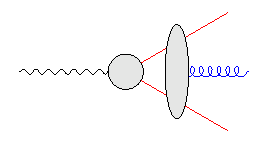
\includegraphics[width=\linewidth]{qcd/A30.pdf}
            \caption{Quark-antiquark antenna, $A_{3}$}
            \vspace{20pt}
        \end{subfigure}
        \begin{subfigure}{0.4\linewidth}
            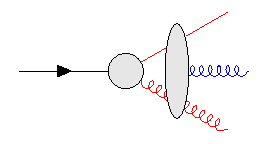
\includegraphics[width=\linewidth]{qcd/D30.pdf}
            \caption{Quark-gluon antenna, $D_{3}$}
            \vspace{20pt}
        \end{subfigure}
        \begin{subfigure}{0.4\linewidth}
            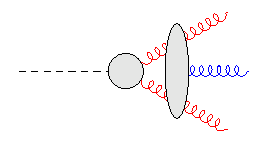
\includegraphics[width=\linewidth]{qcd/F30.pdf}
            \caption{Gluon-gluon antenna, $F_{3}$}
        \end{subfigure}
        \vspace{10pt}
        \caption{Three-parton antenna functions where the loop order
            is implicitly illustrated by the grey circle,
            and the grey ellipse represents all diagrams that give
            rise to the given external states. The hard radiators are
            depicted in red, where as the unresolved parton is coloured
            in blue. External fermion lines have been drawn without
            an arrow to depict the equivalence of quark and antiquark
            antenna functions.}
        \label{fig:antenna}
    \end{figure}

    Below we list the antenna functions relevant
    for multijet production in electron-positron
    annihiliation with a single quark flavour,
    namely the partonic channel $e^{-}e^{+} \rightarrow
    q \bar{q}$ + $n \, g$. The emulation of the NLO QCD K-factors
    of this partonic process is examined in Chapter~\ref{chapter:fame2}.
    For this process we require the $A$, $D$, and $F$ antenna functions,
    which are illustrated in Figure~\ref{fig:antenna}.
    The $i,j,k$ indices will be fixed such that $q = 1$, $\bar{q} = 2$,
    and $g \in \{3, 4, 5\}$ in view of using the
    antenna functions where the momenta
    of partons will have fixed indices in a phase-space
    point represented as an array.

    It will be useful to define the $\mathcal{P}oles$
    and $\mathcal{F}inite$ operators to extract the
    singular and finite contributions from an antenna
    function. However, there are still finite terms
    from $\mathcal{P}oles(X)$ coming from the $\epsilon$-expansion
    of the IR singularity operators given below. Therefore,
    care has to be taken to extract all the finite
    remainders from the antenna functions when trying
    to use them as basis functions for emulating the
    finite part of the one-loop matrix element.

    For the one-loop antenna functions, there are three
    different functions corresponding to the: leading colour,
    subleading colour, and closed quark look contributions.
    It is sufficient to consider the leading colour
    structure in this thesis as the remaining contributions
    are subleading. Ignoring subleading terms in
    colour is equivalent to taking the large $N_{c}$
    limit. For QCD where $N_{c} = 3$, neglecting
    subleading colour terms amounts to an
    approximately 10\% effect.

    The antenna functions have some functions in common,
    namely the singularity operators
    \begin{align}\label{eqn:singularity_operators}
        \begin{split}
        \mathbf{I}_{q\bar{q}}^{(1)}(\epsilon, s_{q\bar{q}}) &= -\dfrac{e^{\epsilon\gamma}}{2\Gamma(1-\epsilon)} \bigg[\dfrac{1}{\epsilon^{2}} + \dfrac{3}{2\epsilon}\bigg] \mathrm{Re}(-s_{q\bar{q}})^{-\epsilon} \, , \\
        \mathbf{I}_{qg}^{(1)}(\epsilon, s_{qg}) &= -\dfrac{e^{\epsilon\gamma}}{2\Gamma(1-\epsilon)} \bigg[\dfrac{1}{\epsilon^{2}} + \dfrac{5}{3\epsilon}\bigg] \mathrm{Re}(-s_{qg})^{-\epsilon} \, , \\
        \mathbf{I}_{gg}^{(1)}(\epsilon, s_{gg}) &= -\dfrac{e^{\epsilon\gamma}}{2\Gamma(1-\epsilon)} \bigg[\dfrac{1}{\epsilon^{2}} + \dfrac{11}{6\epsilon}\bigg] \mathrm{Re}(-s_{gg})^{-\epsilon} \, , \\
        \mathbf{I}^{(1)}_{g\bar{q}}(\epsilon, s_{g\bar{q}}) &= \mathbf{I}_{qg}^{(1)}(\epsilon,s_{g\bar{q}}) \, ,
        \end{split}
    \end{align}
    and dilogarithms which are embedded in the function
    \begin{equation}\label{eqn:R}
        \begin{split}
        R(y, z) = &\log{(y)}\log{(z)} - \log{(y)}\log{(1-y)} - \log{(z)}\log{(1-z)} \\
        &+ \dfrac{\pi^{2}}{6} - \mathrm{Li}_{2}(y) - \mathrm{Li}_{2}(z) \, .
        \end{split}
    \end{equation}
    It will also be useful to introduce the variables $y_{ij} = s_{ij}/s_{ijk}$.

    \subsection{Quark-antiquark antenna functions}
    The quark-antiquark antenna functions are derived by normalising
    the colour-ordered QCD radiative corrections to $\gamma^{*} \rightarrow q \bar{q}$
    at NNLO.
    \subsubsection{Three-parton tree-level antenna function}
    \begin{equation}\label{eqn:A30}
        A_{3}^{0}(1_{q}, 3_{g}, 2_{\bar{q}}) = \dfrac{1}{s_{123}}\left(\dfrac{s_{13}}{s_{23}} + \dfrac{s_{23}}{s_{13}} + 2\dfrac{s_{12}s_{123}}{s_{13}s_{23}}\right) + \mathcal{O}(\epsilon)
    \end{equation}

    \subsubsection{Three-parton one-loop antenna function}
    \begin{align}\label{eqn:A31}
        \mathcal{P}oles\left(A_{3}^{1}(1_{q}, 3_{g}, 2_{\bar{q}})\right) =& \; 2\left(\mathbf{I}_{qg}^{(1)}(\epsilon, s_{13}) + \mathbf{I}_{qg}^{(1)}(\epsilon, s_{23}) \right. \nonumber \\
        &\quad \left. -\mathbf{I}_{q\bar{q}}^{(1)}(\epsilon,s_{123})\right)A_{3}^{0}(1_{q},3_{g},2_{\bar{q}}) \, , \\
        \mathcal{F}inite\left(A_{3}^{1}(1_{q}, 3_{g}, 2_{\bar{q}})\right) =& -\left(R(y_{13}, y_{23}) + \dfrac{5}{3}\log{y_{13}}+\dfrac{5}{3}\log{y_{23}}\right)A_{3}^{0}(1_{q}, 3_{g}, 2_{\bar{q}}) \nonumber\\
        &\quad +\dfrac{1}{s_{123}} + \dfrac{s_{12}+s_{23}}{2s_{123}s_{13}} + \dfrac{s_{12}+s_{13}}{2s_{123}s_{23}} \nonumber \\
        &\quad -\dfrac{s_{13}}{2s_{123}(s_{12}+s_{13})}-\dfrac{s_{23}}{2s_{123}(s_{12}+s_{23})} \nonumber \\
        &\quad +\dfrac{\log{y_{13}}}{s_{123}}\left(2-\dfrac{1}{2}\dfrac{s_{13}s_{23}}{(s_{12}+s_{23})^{2}} + 2\dfrac{s_{13}-s_{23}}{s_{12}+s_{23}}\right) \nonumber  \\
        &\quad +\dfrac{\log{y_{23}}}{s_{123}}\left(2-\dfrac{1}{2}\dfrac{s_{13}s_{23}}{(s_{12}+s_{13})^{2}} + 2\dfrac{s_{23}-s_{13}}{s_{12}+s_{13}}\right) \, .
    \end{align}

    \subsection{Quark-gluon antenna functions}
    The quark-gluon antenna functions are obtained by considering
    the QCD real radiation corrections in the process $\tilde{\chi} \rightarrow \tilde{g} g$.
    \subsubsection{Three-parton tree-level antenna function}
    \begin{equation}\label{eqn:D30}
        \begin{split}
        D_{3}^{0}(1_{q},3_{g},4_{g}) = \dfrac{1}{s_{134}^{2}}&\left(\dfrac{2s_{134}^{2}s_{14}}{s_{13}s_{34}} + \dfrac{2s_{134}^{2}s_{13}}{s_{14}s_{34}} + \dfrac{s_{14}s_{34}+s_{34}^{2}}{s_{13}}\right. \\
        & \left. + \dfrac{s_{13}s_{34}+s_{34}^{2}}{s_{14}} + \dfrac{2s_{13}s_{14}}{s_{34}} + 5s_{134} + s_{34}\right) + \mathcal{O}(\epsilon) \, .
        \end{split}
    \end{equation}
    \subsubsection{Three-parton one-loop antenna functions}
    \begin{align}\label{eqn:D31}
        \mathcal{P}oles\left(D_{3}^{1}(1_{q},3_{g},4_{g})\right) =& \; 2\left(\mathbf{I}_{qg}^{(1)}(\epsilon, s_{13}) + \mathbf{I}_{qg}^{(1)}(\epsilon, s_{14}) + \mathbf{I}_{gg}^{(1)}(\epsilon, s_{34}) \right. \nonumber \\
        &\left. \quad -2\mathbf{I}_{qg}^{(1)}(\epsilon, s_{134}) \vphantom{\mathbf{I}_{gg}^{(1)}} \right) D_{3}^{0}(1_{q},3_{g},4_{g}) \, , \\
        \mathcal{F}inite\left(D_{3}^{1}(1_{q},3_{g},4_{g})\right) =& \; -\left(R(y_{13},y_{34})+R(y_{14},y_{34})+R(y_{13},y_{14}) + \dfrac{5}{3}\log{y_{13}}\nonumber \right. \\
        &\left. \vphantom{\dfrac{1}{1}} \quad + \dfrac{5}{3}\log{y_{14}} + \dfrac{11}{6}\log{y_{34}}\right) D_{3}^{0}(1_{q},3_{g},4_{g}) + \dfrac{1}{3s_{34}} \, .
    \end{align}

    \subsection{Gluon-gluon antenna functions}
    The gluon-gluon antenna functions are obtained from the
    QCD real radiation corrections in the process $H \rightarrow g g$.
    \subsubsection{Three-parton tree-level antenna function}
    \begin{align}\label{eqn:F30}
        F_{3}^{0}(3_{g},4_{g},5_{g}) =& \; \dfrac{2}{s_{345}^{2}}\left(\dfrac{s_{345}^{2}s_{34}}{s_{35}s_{45}} + \dfrac{s_{345}^{2}s_{35}}{s_{34}s_{45}} + \dfrac{s_{345}^{2}s_{45}}{s_{34}s_{35}} \right. \nonumber \\
        &\left. \vphantom{\dfrac{s_{345}^{2}s_{34}}{s_{35}s_{45}}} \quad \quad +\dfrac{s_{34}s_{35}}{s_{45}} + \dfrac{s_{34}s_{45}}{s_{35}} + \dfrac{s_{35}s_{45}}{s_{34}} + 4s_{345} + \mathcal{O}(\epsilon) \right) \, .
    \end{align}
    \subsubsection{Three-parton one-loop antenna functions}
    \begin{align}\label{eqn:F31}
        \mathcal{P}oles\left(F_{3}^{1}(3_{g},4_{g},5_{g})\right) =& \; 2\left(\mathbf{I}_{gg}^{(1)}(\epsilon,s_{34}) + \mathbf{I}_{gg}^{(1)}(\epsilon,s_{35}) + \mathbf{I}_{gg}^{(1)}(\epsilon,s_{45}) \right. \nonumber \\
        &\left. \quad -2\mathbf{I}_{gg}^{(1)}(\epsilon,s_{345})
        \right) F_{3}^{0}(3_{g},4_{g},5_{g}) \, , \\
        \mathcal{F}inite\left(F_{3}^{1}(3_{g},4_{g},5_{g})\right) =& -\left(R(y_{34},y_{35}) + R(y_{35},y_{45}) + R(y_{34},y_{45}) \vphantom{\dfrac{1}{1}} \right. \nonumber \\
        &\left. \quad + \, \dfrac{11}{6}\log{y_{34}} + \dfrac{11}{6}\log{y_{35}} + \dfrac{11}{6}\log{y_{45}} \right) F_{3}^{0}(3_{g},4_{g},5_{g}) \nonumber \\
        & \quad + \dfrac{1}{3s_{34}} + \dfrac{1}{3s_{35}} + \dfrac{1}{3s_{45}} + \dfrac{1}{3s_{345}} \, .
    \end{align}
    \subsection{Limiting behaviour of antenna functions}
    Examining (\ref{eqn:A30}) more closely, it becomes clear
    that the correct IR behaviour is exhibited by the antenna
    function. The first two terms correspond to the gluon
    going collinear with the quark and antiquark. The final
    term encapsulates singularity in the limit of the gluon
    going soft.

    The other antenna functions have similar limiting behaviour,
    collapsing to the single collinear and soft splitting functions
    in the relevant regions of phase-space.

    Utilising this property of the antenna functions, and the fact
    that they naturally interpolate between the soft and collinear
    limits due to being derived from physical matrix elements,
    they can be used as a set of basis functions for approximating
    matrix elements. This will be explored in Chapter~\ref{chapter:fame2}.
\end{document}
